\documentclass[fra, final]{anthology-ch}      % pour la soumission

% CHARGER LES PACKAGES LaTeX
\usepackage{booktabs}
\usepackage{graphicx}
\usepackage{subcaption} 

\title{\texorpdfstring{Des émotions au fil du récit : \\ \texttt{fabula}, un package pour analyser les textes francophones par Transformers}{Des émotions au fil du récit : fabula, un package pour analyser les textes francophones par Transformers}}

\author[1,2]{Florian Cafiero}[
  orcid=0000-0002-1951-6942,
  email=florian.cafiero@chartes.psl.eu,
  corresponding=true
]

\author[3]{Alexandre Lionnet}[
  orcid=0009-0002-1131-8447,
  email=alexandre.lionnet@ephe.psl.eu
]

% AFFILIATIONS
\affiliation{1}{LRE, Ecole Pour l'Informatique et les Techniques Avancées (EPITA), Paris, France}
\affiliation{2}{École nationale des chartes, Université Paris Sciences \& Lettres (PSL), Paris, France}
\affiliation{3}{École Pratique des Hautes Études, Université Paris Sciences \& Lettres (PSL), Paris, France}

% MOTS-CLÉS
% Fournissez un ou plusieurs mots-clés séparés par des virgules
% en utilisant les commandes suivantes
\keywords[fra]{python, analyse de sentiments, détection d'émotions, BERT, études littéraires computationnelles}
\keywords[eng]{python, sentiment analysis, emotion detection, BERT, computational literary studies}

% MÉTADONNÉES DE LA PUBLICATION
% Ces champs seront remplis lors de la publication ; 
% ils peuvent être laissés par défaut lors de la soumission
\pubyear{2026}
\pubvolume{4}
\pagestart{72}
\pageend{78}
\paperorder{9}
\conferencename{Actes de la Conférence Humanistica}
\conferenceeditors{Serena Crespi, Simon Gabay, Martin Grandjean, Ariane Pinche, Marie Puren et Léa Saint-Raymond}
\doi{10.63744/hHyKtxX4Iu6S}
\customhead{}

\addbibresource{bibliography.bib}




\begin{document}

\maketitle

\begin{abstract}
Computational emotion analysis has become an established tool in computational literary studies for describing and comparing narratives. However, the solutions currently available for French remain limited and often rely on fixed lexicons that are not very robust to context, such as polysemy, negation, or irony, and that are difficult to relate back to the text in a fine-grained way. We present here \texttt{fabula-fr}, a Python package designed for emotion analysis in Francophone narratives. It is based on Transformer models while retaining a simple and reproducible pipeline. \texttt{fabula} offers several segmentation and smoothing strategies, an “in-context” mode to stabilize the analysis of long texts, preservation of probabilistic distributions, configurable smoothed arcs, and procedures providing \textit{a minima} explainability for classification choices. Our article situates these design choices within the state of the art and proposes an agenda for validation and extension.
\end{abstract}

\section{Introduction}

L'ambition de quantifier l'évolution émotionnelle d'un récit — ce que le formalisme russe nomme le \textit{syuzhet} — est devenue l'un des chantiers les plus visibles de la « lecture distante » (\textit{distant reading}). L'objectif est notamment de vérifier empiriquement l'hypothèse formulée par l'écrivain Kurt Vonnegut, selon laquelle les histoires suivent des courbes émotionnelles simples et universelles, telles que « l'homme dans un trou » (\textit{Man in a Hole}) ou « Cendrillon » \parencite{vonnegut2005}.

Cependant, la traduction de cette intuition littéraire en algorithmes soulève des questions méthodologiques fondamentales : que mesure-t-on exactement ? à quelle échelle du texte ? avec quelle comparabilité entre œuvres ? et avec quel niveau d’interprétabilité pour permettre le retour au texte ? Cet article procède en trois temps : (1) un état de l’art centré sur les usages de l’analyse des émotions en humanités numériques ; (2) une discussion des choix méthodologiques qu’implique l’opérationnalisation de ces usages, à partir du cas canonique de \texttt{syuzhet} \parencite{jockers2015revealing} ; (3) la présentation de \texttt{fabula}, un package Python reposant sur des modèles Transformer (plutôt que sur des lexiques fixes), et des perspectives de validation et d’extension.

\section{Usages et choix méthodologiques : de la fouille de corpus aux arcs narratifs}

La littérature récente mobilise l’analyse des émotions et du sentiment comme un instrument de description, de comparaison et d’exploration des récits. De récentes synthèses proposent des typologies convergentes de ces usages \parencite{kimklinger2021survey}. L’intérêt de ce champ est qu’il articule des objectifs interprétatifs (décrire, comparer, naviguer, inférer) à des choix techniques très concrets (segmentation, représentation du signal, modèles, lissage, évaluation). En pratique, ces choix deviennent d’autant plus visibles que l’on cherche à produire des sorties comparables (entre œuvres, genres, périodes) et suffisamment interprétables pour permettre un retour au texte.

Un premier ensemble de travaux s’inscrit dans une logique de fouille de corpus et de navigation dans des collections : il s’agit d’indexer des textes à partir d’affects dominants, de repérer des régularités comme les « fins heureuses » \parencite{zehe2016happyendings}, ou de construire des profils émotionnels rendant des œuvres comparables à grande échelle \parencite{kakkonen2011sentiprofiler}. Cette orientation prolonge aussi des discussions plus anciennes sur l’usage de méthodes de classification et de regroupement pour l’étude littéraire \parencite{yu2008litstudy}. À ce niveau, une première décision méthodologique est centrale : l’unité d’analyse. Indexer un roman « globalement » ou indexer des segments (chapitres, paragraphes, phrases) ne produit pas la même information, ni les mêmes possibilités de navigation. Le choix de segmentation conditionne aussi la sensibilité aux effets de style, aux scènes dialoguées, ou aux ruptures narratives.

Ces usages de description se prolongent vers une approche plus formelle des dynamiques narratives : plutôt que d’assigner une tonalité globale à un roman, l’enjeu devient de suivre l’évolution du signal affectif et d’identifier des trajectoires récurrentes, comme l’ont illustré des analyses à grande échelle des arcs émotionnels \parencite{reagan2016emotionalarcs}. Dans la même veine, plusieurs travaux ont examiné le lien entre développement émotionnel et genres \parencite{kimpadoklinger2017genres} ou discuté l’existence de trajectoires « prototypiques » selon les sous-genres \parencite{kimpadoklinger2017prototypes}. L’arc narratif met alors au premier plan un second choix méthodologique : comment transformer une série de scores en une forme comparable. Deux opérations reviennent fréquemment : (1) le ré-échantillonnage (ramener des textes de longueurs différentes à une grille commune), et (2) le lissage (réduire le bruit local pour privilégier la tendance). Ces opérations répondent à un objectif comparatif et de lisibilité, mais elles introduisent des paramètres (taille de fenêtre, intensité du lissage, méthode de filtrage) qui doivent être rendus explicites pour éviter les glissements d’interprétation.

Dans ce contexte, certaines chaînes de traitement se sont imposées comme des solutions canoniques parce qu’elles standardisent ces décisions et les rendent facilement reproductibles. Le package R \texttt{syuzhet} \parencite{jockers2015revealing} joue ici un rôle important : il propose un pipeline « texte $\rightarrow$ série $\rightarrow$ arc » et popularise l’idée d’une visualisation stable des dynamiques affectives. Ses choix techniques typiques — extraction lexicale à partir de dictionnaires (dont le \textit{NRC Word-Emotion Association Lexicon} \parencite{mohammad2013}) et lissage du signal (initialement via FFT, puis alternatives) — ont contribué à diffuser une pratique comparatiste clé-en-main. Mais cette standardisation rend également visibles les points sensibles du protocole : d’une part, une controverse mathématique a porté sur l’usage de la FFT et les artefacts de bord induits sur un signal fini (phénomène de Gibbs) \parencite{swafford2015}, ce à quoi ont répondu des variantes (moyennes mobiles, LOESS, DCT) \parencite{jockers2015requiem} ; d’autre part, l’approche par dictionnaire reste structurellement limitée par sa faible prise en compte du contexte, notamment face à la polysémie, à la négation et à l’ironie, difficultés classiques des méthodes \textit{bag-of-words} \parencite{pang2008}. Autrement dit, les débats autour de \texttt{syuzhet} ne sont pas seulement « un cas » : ils cristallisent des questions générales sur ce que mesure un score affectif, à quelle échelle, et avec quelle robustesse.

Une partie de la recherche a transposé ces méthodes à des corpus diachroniques ou historiques, où les contraintes se renforcent : variation linguistique, décalage sémantique, bruit d’OCR et nécessité de protocoles d’évaluation adaptés \parencite{sprugnoli2016historical}. Dans ces contextes, la comparabilité des signaux affectifs devient une hypothèse à tester plutôt qu’un acquis, comme le montrent des travaux sur la fiction à long terme \parencite{morinacerbi2017emotionality}. Cela souligne un troisième choix méthodologique : l’alignement entre objectif et procédure d’évaluation. Un pipeline utile pour la navigation exploratoire peut être insuffisant pour des inférences diachroniques, où l’on attend une stabilité sémantique et des contrôles plus stricts.

Enfin, un autre ensemble de travaux se structure autour d’analyses centrées sur les personnages : l’objectif est d’attribuer des affects à des entités et de décrire des relations émotionnelles dirigées (qui ressent quoi envers qui). Des approches pionnières ont exploré l’extraction de réseaux affectifs dans des corpus dramatiques \parencite{nalisnickbaird2013shakespeare} ; d’autres ont proposé de cartographier des relations émotionnelles au fil d’un récit \parencite{jhavarmirza2018emofiel}. Plus récemment, l’annotation de rôles sémantiques de l’émotion a contribué à stabiliser ce type d’analyse \parencite{kimklinger2018whofeelswhat}, et des modèles ont été entraînés pour classifier explicitement des relations émotionnelles entre personnages \parencite{kimklinger2019relationships}. Ici, la question méthodologique dominante est celle de l’attribution (à quel personnage associer l’émotion) et du retour au texte : pour être utile en narratologie, le signal doit rester traçable, segmentable et justifiable.

À ces familles s’ajoutent des usages transversaux où le signal affectif sert de variable secondaire dans des analyses critiques et sociologiques : il peut éclairer des phénomènes macroscopiques, comme des hiérarchies de genre dans la fiction contemporaine \parencite{kraicerpiper2019socialcharacters} ou des effets de catégorisation associés aux « livres de femmes » \parencite{koolen2018womensbooks}. Dans des travaux plus appliqués, l’émotion peut aussi servir au filtrage, à la recherche ciblée, ou à l’étude de configurations discursives spécifiques \parencite{cafiero2025riddle,zribi2026tictalk,lionnet2025makes, lionnet2026nevercare}.

Ces usages convergent vers un constat : les approches lexicales ont eu le mérite de stabiliser des pipelines reproductibles, mais elles atteignent rapidement une limite sémantique — la difficulté à représenter le contexte — dès que l’on veut interpréter finement des segments ou comparer des œuvres hétérogènes. L’émergence des modèles de langue pré-entraînés basés sur l’architecture Transformer, tels que BERT \parencite{devlin2018bert}, modifie précisément ce point : au lieu d’associer un mot à une valence fixe, le modèle produit des représentations contextualisées où le sens dépend du voisinage syntaxique et sémantique. Pour les humanités numériques, l’enjeu n’est pas de remplacer un outil par un autre, mais de conserver des sorties utiles aux usages établis (navigation, arcs, comparaisons) tout en rendant explicites les décisions qui conditionnent la robustesse et l’interprétabilité du signal \parencite{kimklinger2021survey}.

\section{Le package \texttt{fabula} : fonctionnalités déduites des usages et fonctionnement actuel}

Le package \texttt{fabula} vise à décrire l’évolution des émotions ou du sentiment tout au long d’un texte narratif. Son choix central est de conserver le geste opératoire qui a fait le succès de \texttt{syuzhet} (texte $\rightarrow$ série $\rightarrow$ arc), tout en remplaçant l’approche lexicale par des modèles de langue contextuels. Concrètement, le pipeline se veut minimal et transparent : découper le texte en segments, attribuer une distribution de scores à chaque segment à l’aide d’un modèle de langue, puis transformer cette série de scores en un « arc » lissé comparable d’un texte à l’autre. \texttt{fabula} propose deux modes d’analyse — sentiment (positif vs négatif) et émotion (joie, tristesse, etc.) — afin de s’adapter aux traditions de recherche déjà établies (valence globale ou répartition d’affects).

%Schéma

\subsection{Segmentation : choix du niveau d’observation}

Le découpage du texte est décisif : il détermine la granularité de lecture, et conditionne la plupart des usages recensés (exploration de collections, arcs et genres, textes longs, personnages). \texttt{fabula} fournit quatre stratégies. Par défaut, les documents sont segmentés par phrases. Ils peuvent également être traités paragraphe par paragraphe, ou en suivant des fenêtres de tokens glissantes (algorithme roulant).

\subsection{Le mode « in-context » : réinjecter du contexte dans les textes longs}

Les \texttt{Transformers} offrent un avantage net par rapport aux approches lexicales, mais ils restent contraints par une limite de longueur d’entrée : ils ne « lisent » qu’un nombre fini de tokens. Cette contrainte peut nuire à la compréhension contextuelle d’un passage, surtout dans les textes longs. En l’absence de modèles francophones de type Longformer entraînés spécifiquement pour l’émotion ou le sentiment, \texttt{fabula} propose un mode alternatif à évaluer.

L’intuition est la suivante : si une phrase isolée diverge fortement du ton général d’un passage, il est possible qu’elle doive être interprétée à la lumière du contexte (ironie, contraste, rupture narrative). Autrement dit, une phrase très négative au milieu d’un passage globalement positif ne devrait pas nécessairement inverser l’évaluation globale.

Le mode « in-context » combine donc deux niveaux de lecture. Le texte est d’abord découpé en phrases (segments fins), puis en grands blocs de tokens (segments larges). Chaque niveau est scoré séparément par le modèle. Ensuite, pour chaque phrase, \texttt{fabula} calcule une moyenne pondérée des scores des blocs voisins : les blocs proches comptent davantage que les blocs lointains, afin d’injecter du contexte global sans effacer la dynamique locale. Enfin, les scores « phrase » et « bloc » sont fusionnés via un poids réglable (par défaut 0{,}3 pour les blocs). Ce mécanisme vise à conserver la finesse de l’analyse locale tout en stabilisant l’interprétation globale des textes longs.

\subsection{Scorage probabiliste : conserver l’incertitude}

Au lieu d’un score binaire, chaque segment reçoit une distribution de probabilités sur les étiquettes du modèle (sentiments ou émotions). Cette distribution complète est conservée, ce qui permet des analyses plus fines que la simple classe gagnante (par exemple, suivre la compétition entre « tristesse » et « peur »). Pour les arcs « scalarisés », \texttt{fabula} calcule ensuite un score synthétique : une valence (positif – négatif) en mode sentiment, ou la probabilité maximale en mode émotion. Ce choix maintient un lien direct avec la sortie brute du modèle, tout en restant interprétable pour un public non spécialiste.

\begin{figure}[ht]
    \centering
    \begin{subfigure}{0.45\textwidth}
        \centering
        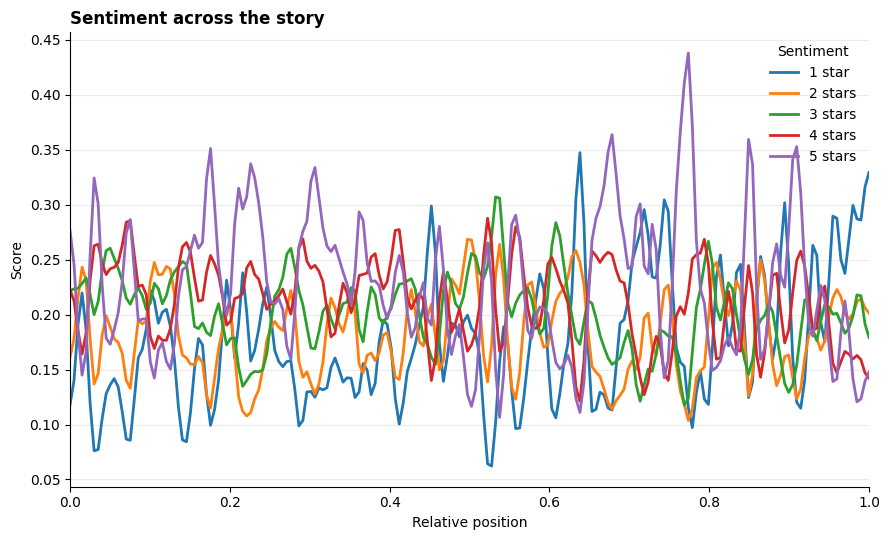
\includegraphics[width=\textwidth]{img/stendhal_sentiments.png}
        \caption{Exemple de répartitions des résultats de valence à travers \textit{Le rouge et le Noir} de Stendhal. Ré-échantillonnage à 200 points.}
        
    \end{subfigure}
    \hfill
    \begin{subfigure}{0.45\textwidth}
        \centering
        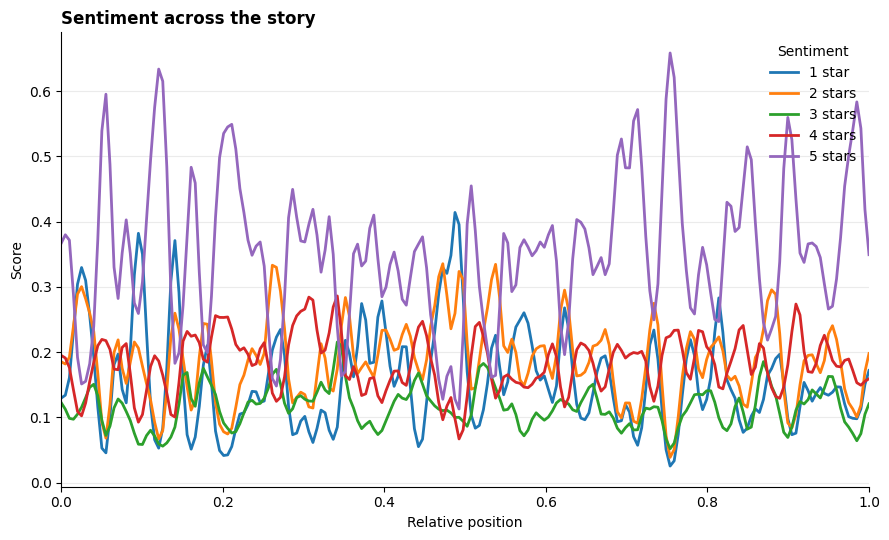
\includegraphics[width=\textwidth]{img/tesson_series.png}
        \caption{Exemple de répartitions des résultats de valence à travers \emph{Dans les Forêts de Sibérie} de Sylvain Tesson. Ré-échantillonnage à 200 points.}
        
    \end{subfigure}
    \end{figure}
\hfill
\subsection{Arc narratif lissé : comparabilité et lisibilité}

Une narration n’est pas un signal régulier ; \texttt{fabula} transforme donc la série irrégulière de scores en un nombre fixe de points (ré-échantillonnage) et applique un lissage configurable (moyenne mobile, gaussien ou aucun lissage). Ce choix est justifié par un objectif comparatif : rendre des textes de longueurs différentes lisibles sur une même échelle, tout en limitant le bruit local. L’utilisateur peut garder la série brute ou ajuster la quantité de lissage selon son protocole analytique.



\begin{figure}[ht]
    \centering
    \begin{subfigure}{0.45\textwidth}
        \centering
        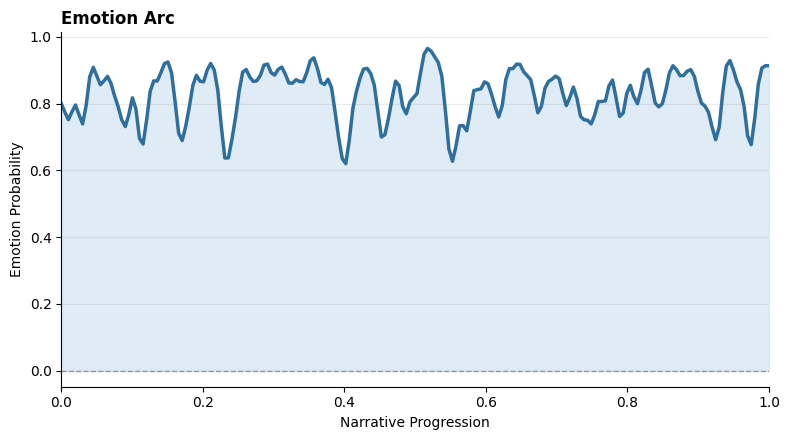
\includegraphics[width=\textwidth]{img/stendhal_emotion_narrative_arc.png}
        \caption{Exemple d'un arc narratif produit à partir des scores d'émotion sur \textit{Le Rouge et le Noir} de Stendhal. Ré-échantillonnage à 200 points, lissage gaussien.}
        
    \end{subfigure}
    \hfill
    \begin{subfigure}{0.45\textwidth}
        \centering
        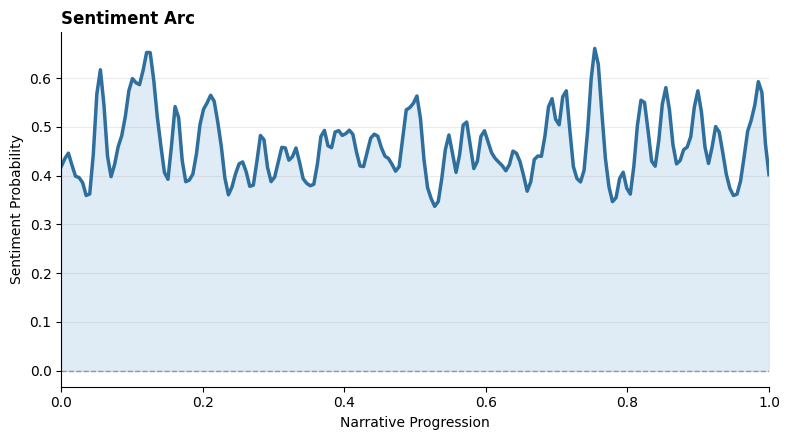
\includegraphics[width=\textwidth]{img/tesson.png}
        \caption{Exemple d'un arc narratif produit à partir des scores de sentiment sur \textit{Dans les Forêts de Sibérie} de Sylvain Tesson. Ré-échantillonnage à 200 points, lissage gaussien.}
        
    \end{subfigure}

\end{figure}

\subsection{Interprétabilité : expliquer quels mots influencent la décision}

Pour répondre à la critique fréquente des « boîtes noires », \texttt{fabula} inclut une procédure d’explicabilité simple : pour un segment donné, il mesure l’impact de chaque token en le supprimant puis en recalculant la probabilité de la classe cible. Le résultat est une liste de tokens accompagnés d’une variation de probabilité (delta), ce qui identifie les mots qui contribuent le plus à la décision du modèle. L’option est accessible via l’API (et exposée côté CLI), ce qui permet de l’utiliser comme outil d’analyse qualitative, ou comme justification méthodologique dans un protocole DH. Cette méthode a l’avantage d’être directement compréhensible pour un lecteur non spécialiste : « retirer tel mot fait baisser la confiance du modèle ». Nous soulignons toutefois qu’il s’agit d’une heuristique exploratoire : la suppression d’un token (souvent un sous-mot) peut modifier l’encodage global et ne constitue pas, en soi, une attribution causale stable. Ces scores doivent être interprétés qualitativement et triangulés avec d’autres indices.

\subsection{Accès et formats : reproductibilité pratique}

Enfin, \texttt{fabula} est utilisable en ligne de commande ou via une API Python. Les sorties sont en CSV ou JSON : soit un tableau de scores par segment (\texttt{score}), soit un arc lissé (\texttt{arc}). Les modèles par défaut sont francophones, mais tout modèle Hugging Face de classification séquentielle peut être fourni, ce qui rend l’outil adaptable à d’autres langues ou jeux d’étiquettes, sans modifier le code de base.

\section{Perspectives}

Cette première version de \texttt{fabula} propose une première étape pour remplir les usages que nous avons pu identifier. Mais plusieurs chantiers restent ouverts.

\begin{enumerate}
    \item \emph{Entraîner de nouveaux modèles} mieux adaptés à la détection d'émotions et de sentiments pour le français, pour différentes époques. L'offre est pour l'instant trop restreinte et pas toujours adaptée.
    \item \emph{Évaluer le mode « in-context » :} comparaison systématique avec le mode standard, analyses de sensibilité (poids des blocs, taille des fenêtres) et critères d’évaluation alignés avec les objectifs (robustesse des arcs, cohérence interprétative).
    \item \emph{Traiter structurellement la contrainte de longueur :} exploration de modèles alternatifs, en particulier des architectures à long contexte, et formalisation de recommandations pratiques (tailles de segments, fenêtres, lissage) pour les textes longs après expérimentations sur des corpus littéraires.
    \item \emph{Étendre à d'autres langues} : inclure la gestion par défaut de différents modèles d'autres langues adaptées au contexte littéraire.
\end{enumerate}

\section*{Disponibilité des données}

Le code source du package \texttt{fabula} et sa documentation sont disponibles en ligne :
\href{https://github.com/floriancafiero/fabula}{https://github.com/floriancafiero/fabula}. Le package est disponible sur pypi: \href{https://pypi.org/project/fabula-fr}{https://pypi.org/project/fabula-fr}.

\printbibliography

\appendix

\end{document}